		% !TEX root =  reply_letter.tex
		\clearpage
		\section*{Response to 1st Referee's Comments}
		We would like to thank the Referee for their constructive comments, which have allowed us to considerably improve our paper. The main differences of the new version of the manuscript compared to the previous one can be found in Study Population section of the paper.

		\begin{enumerate}

		    \item \underline{Risk calculator for clinicians for bringing the concept to practice}

		    We thank the Referee for their suggestion of a risk calculator. We have already developed a web-application for this purpose (Figure \ref{fig:webapp}). In this web-application doctors can load patient data via CSV files (and other formats such as SPSS files). To aid in shared decision making, the web-application not only estimates the cumulative risk of cancer progression at the current visit, but also on future visits. These estimates are time-dynamic, that is, they get updated as additional patient data is collected over time. In addition, patient-specific fitted PSA and DRE profiles and their future predictions are also provided. 

		    \begin{figure}[!htb]
	    		\centerline{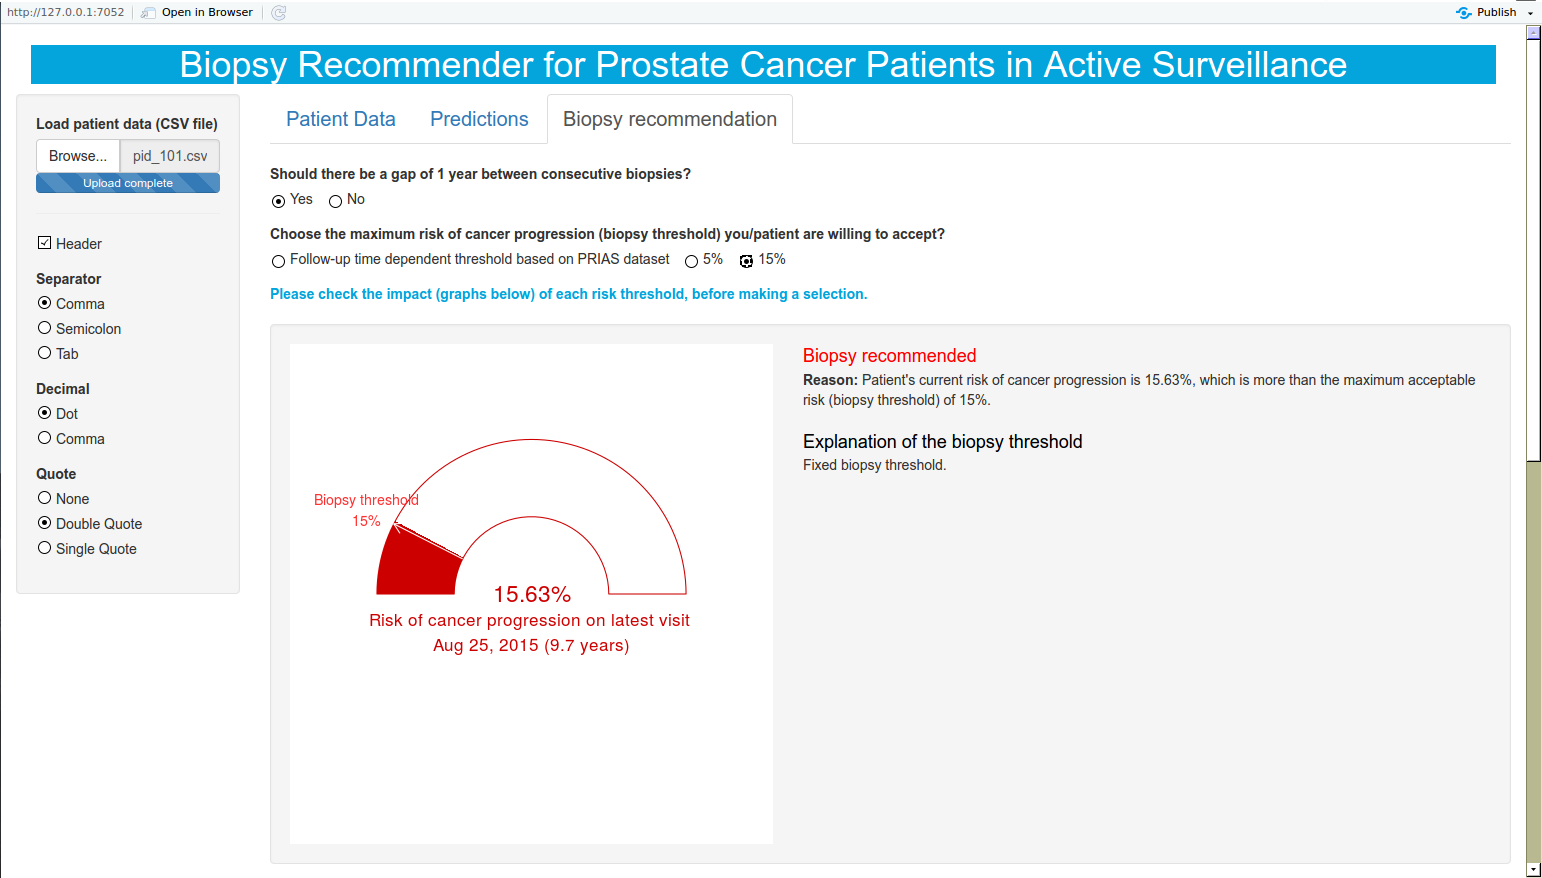
\includegraphics[width=0.8\columnwidth]{../images/webapp.png}}
				\caption{Web-based risk calculator for prediction of risk of prostate cancer progression.}
				\label{fig:webapp}
			\end{figure}

			Although the web-application is ready, our model requires further validation. To this end, we are currently validating it using active surveillance data from the GAP3 database \citep{bruinsma2018movember}. The GAP3 database consists of patient data from multiple active surveillance cohorts around the world. Based on the current validation results so far, we expect the web-application to be also useful in other cohorts which are similar to PRIAS.

			\item \underline{Model robustness to Gleason score misclassification}

			We thank the Referee for motivating us to check the robustness of our model against Gleason score misclassification. A biopsy Gleason score can be misclassified to be less than the pathological score (prostatectomy), or vice versa. Ignoring such misclassification will affect the parameter estimates as well risk predictions. 

			\textbf{Impact of Gleason misclassification on parameter estimates:}
			The impact of Gleason misclassification on parameter estimates depends upon the misclassification rate. Higher rates of misclassification may lead to a larger bias in the parameter estimates. In general, there is little consensus on the rate of Gleason misclassification \citep{cookson1997, Ploussard2010,Lattouf2002, Melia2006, Pinthus2006}. As is likely, the Gleason misclassification rate may vary between cohorts. Consequently, the right approach will be to find Gleason misclassification rates in the PRIAS program and utilize them to model pathological Gleason score as an outcome in our model \citep{balasubramanian2003estimation, coley2017}. However, in the PRIAS dataset such information is available only for the patients who opted for radical prostatectomy. The Gleason misclassification rate in such patients is roughly 4.5\%. This rate is much less than the misclassification rates reported in studies cited above. We currently lack information on misclassification rate in random sample of the population (likely higher than 4.5\%). Hence, accounting for it in the model is currently not feasible. Thus, the parameter estimates that we reported are only valid for the clinically relevant endpoint of upgrade in biopsy Gleason score. 

			%\textbf{Impact of Gleason misclassification on risk prediction:}
			%When a Gleason score of 7 or more is misclassified as a Gleason score of 6 or less, the patient is removed from active surveillance for treatment. Hence predictions from our model may not be used afterwards. We next discuss the alternative scenario wherein a Gleason score of 7 or more is misclassified as a Gleason score of 6 or less. In this case the patient remains in active surveillance and our model may be used to schedule biopsies.

			%\textit{Model utilizes multiple sources of information:} The personalized risk of cancer progression for a patient $j$ depends upon four sources of information, namely the time of the latest negative biopsy $t$, the repeated measurements  $\mathcal{Y}_{pj}(s)$ and $\mathcal{Y}_{dj}(s)$ of PSA (prostate-specific antigen) and DRE (digital rectal examinations), respectively, and the training data $\mathcal{D}_n$. That is the model does not rely completely on the observed Gleason score. This is evident by the following formula for the risk of cancer progression at a time $s$:
			%\begin{equation}
			%	\label{eq:dynamic_risk_prob}
			%	R_j(s \mid t) = \mbox{Pr}\big\{T^*_j \leq s \mid T^*_j > t, \mathcal{Y}_{dj}(s), \mathcal{Y}_{pj}(s), \mathcal{D}_n\big\}, \quad s \geq t,
			%\end{equation}
			%where $T^*_j$ is true time of cancer progression (Gleason upgrade). 

			%\textit{Impact of 100\% misclassification rate on risk prediction:} In order to check the robustness of predictions against Gleason misclassification, we conducted a set of simulations. The setup of these simulations was same as that of the main simulation study reported in our manuscript. Let us assume that we schedule a biopsy for all patients at the exact time of their cancer progression $T^*_j$. We then assume that we incorrectly obtain a Gleason score less than 7 for all such patients, that is, we have a 100\% misclassification rate. Consequently, these patients will remain in active surveillance and will be invited at future follow-up time points $s > T^*_j$. The risk of cancer progression at these future time points is given by Equation~(\ref{eq:dynamic_risk_prob}), with $t=T^*_j$. We then make a decision of biopsy at the future time points based on two different risk cutoffs, namely 5\%, 10\%. We assume that the urologist will correctly classify the Gleason score on this second biopsy. Consequently, the delay in detection of cancer progression is the difference between the time of the second biopsy and the true time of cancer progression (at which a biopsy was done, but Gleason score was misclassified). 

			%In the aforementioned scenario, we observed that for a risk cutoff of 5\% the delay in detection of cancer progression (years) is median:~0.6,~IQR:~0.3--1.0. This is similar to the delay we observe in the main simulation study for this cutoff (median:~0.6,~IQR:~0.3--0.9) wherein we ignore Gleason misclassification. For a risk cutoff of 10\% the delay in years is median:~1.0,~IQR:~0.6--1.8. In this case the third quartile of the delay is much more than the case wherein we ignore Gleason misclassification (median:~0.7,~IQR:~0.3--1.0). In AS, a delay in the detection of cancer progression around 12 to 14 months is assumed to be unlikely to substantially increase the risk of adverse downstream outcomes \citep{inoue2018comparative,carvalho}. While the third quartile of the delay with a 10\% cutoff is 7 months above this limit, this result is based on an extreme scenario of 100\% misclassification. In reality Gleason misclassification rates are much lower, and rates as high as 50\% (random classification) are only likely when pathological Gleason score is exactly 7 \citep{cookson1997, Ploussard2010,Lattouf2002, Melia2006, Pinthus2006}. In light of these arguments, a 5\% to 10\% cutoff may still be useful to decide biopsies.

			\item \underline {Typos on page 6, line 44}
			
			We thank the Referee for pointing out the error. The new text is:
			
			\begin{shadequote}
				\textbf{Data Accessibility:} The PRIAS database is not openly accessible. However, access to the database can be requested on the basis of a study proposal approved by the PRIAS steering committee. The website of the PRIAS program is \url{www.prias-project.org}.
			\end{shadequote}
			
		\end{enumerate}

